\documentclass[%
12pt, %
final, % 
oneside, % 
onecolumn, %  
centertags]{article} % относится к классу article и размер шрифта 12 пунктовб, {article: статья, report: отчеты и диссертации, book: книга, letter: письмо}

% \usepackage{fontspec}
 
% \setmainfont{Times New Roman}

% \documentclass[a4paper, 12pt]{report}

\topmargin= -30pt % насколько сверху будет страница
\textheight= 650pt


\usepackage[utf8]{inputenc} % задает кодировку, utf-8 кодировка, включающая в себя знаки почти всех языков мира
\usepackage[english]{babel} % подключает необходимые языки, основным языком является английский

\selectlanguage{english} % настройки будут на английском, но писать будет на русском

\usepackage{euscript}
\usepackage{supertabular}

\renewcommand{\baselinestretch}{1.0} 

\usepackage[colorlinks=true,linkcolor=blue,unicode=true,urlcolor = blue]{hyperref} %hypered
\usepackage[pdftex]{graphicx} % для графики

\usepackage{amsthm, amssymb, amsmath, amsfonts} % математический пакет, математические шрифты
\usepackage{textcomp}
\usepackage[noend]{algorithmic}
\usepackage[ruled]{algorithm}
\usepackage{lipsum}
\usepackage{indentfirst}
\usepackage{babel}
\usepackage{pgfplots}
\usepackage{setspace}
\usepackage{xcolor}
\usepackage{hyperref}
\usepackage{subfigure}

\setcounter{secnumdepth}{5}
\setcounter{tocdepth}{5}
\newcommand\simpleparagraph[1]{%
  \stepcounter{paragraph}\paragraph*{\theparagraph\quad{}#1}}
\usepackage{listings}
% \usepackage{xcolor}
%\usepackage{minted}

\lstset { %
     language=C++,
     backgroundcolor=\color{black!5}, % set backgroundcolor
     basicstyle=\footnotesize,% basic font setting
}


\linespread{1.0} 
\setlength{\parindent}{2.4em}
\setlength{\parskip}{0.1em}

\pgfplotsset{compat=1.9}
\pgfplotsset{model/.style = {blue, samples = 100}} 
\pgfplotsset{experiment/.style = {red}}

\theoremstyle{plain}
\binoppenalty=10000

\newtheorem{theorem}{Theorem}[section] % theorem

\theoremstyle{definition}
% \newtheorem{definition}{Определение}[subsection]
\newtheorem{definition}{Definition}[subsection]

\theoremstyle{remark}
% \newtheorem{remark}{Замечание}[section]

% \newtheorem{corollary}{Следствие}

% \newtheorem{proposition}{Proposition}

% \newtheorem{example}{Пример}

% \newtheorem{lemma}{Лемма}[section]

\renewcommand*{\proofname}{Proof}

\graphicspath{ {./images/} }


% \usepackage{amsmath,amsfonts,amssymb, setspace}  % Разнообразные математические команды и значки
% \usepackage{indentfirst}     % Отступ в первом абзаце

% \pagestyle{empty}
\usepackage[left=2.5cm, right=1.5cm, top=2.5cm, bottom=2.5cm]{geometry}
\usepackage[medium]{titlesec}
\usepackage{graphicx}
% \graphicspath{ {./images/} }

\begin{document}

	\begin{titlepage} 
		\begin{center}
		\textbf{}\\[2.0cm]
		\LARGE FEDERAL STATE AUTONOMOUS EDUCATIONAL INSTITUTION OF HIGHER EDUCATION \\[0.5cm]
		\Large ITMO UNIVERSITY \\[3cm]
		\LARGE Report\\
		\Large MPI. Assignments $18-19$ \\
		\Large Parallel algorithms for the analysis and synthesis of data \\[4cm]


		\begin{flushright}
		Performed by\\
		Aleksandr Shirokov\\
		J4133c\\
		Accepted by\\
		Petr Andriushchenko

		Deadline: 25.12.21
		\end{flushright}

		\vfill 

		{\Large {St. Petersburg}} \par
		{\Large {2021}}
		\end{center} 
	\end{titlepage}

\tableofcontents
\newpage


\section{Assignments}

\subsection{Assignment 18. MPI. Operations with communicators. Renumbering processes.}

\subsubsection{Formulation of the problem}

To complete the task, you need to create and compile two programs: Master (\textsc{master.o}) and Slave (\textsc{slave.o}). 
The Master should start the worker, so be careful with the names of the executable files.

Launch the master via the mpiexec command for one process.

Startup example: \textsc{mpiexec -n 1 ./master.o}.

Understand the new functions in \textsc{Assignment18\_master.c} and \textsc{Assignment18\_slave.c} and explain programs 
execution.

Add a third process, which will transfer from the slave processes to the master the number of running 
processes, the master should receive and display


\subsubsection{Example of launch parameters and output. Detailed description of solution}

Code for \textbf{assignment 18} are \href{https:\//github.com/aptmess/parallel_algorithms/blob/master/HT/hw_mpi/Assignment18_master.c}{here}(master) and \href{https:\//github.com/aptmess/parallel_algorithms/blob/master/HT/hw_mpi/Assignment18_slave.c}{here}(slave).

Compilation example: 

\begin{enumerate}
	\item \textsc{mpic++ -o ./cpf/18\_master.o Assignment18\_master.c}
	\item \textsc{mpic++ -o ./cpf/18\_slave.o Assignment18\_slave.c}
\end{enumerate}

Launch example: \textsc{mpirun --oversubscribe -np 1 ./cpf/18\_master.o}

\begin{center}
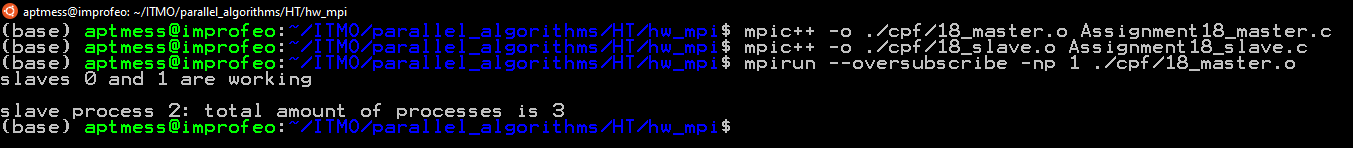
\includegraphics[scale=0.5]{18.png}
\end{center}

Let's move to the the code and explain how it works.

\begin{center}
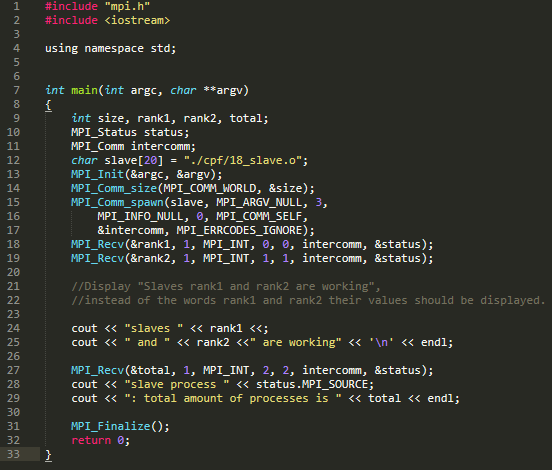
\includegraphics[scale=1.1]{18.master.code.png}

Assignment 18 - master code
\end{center}

\begin{center}
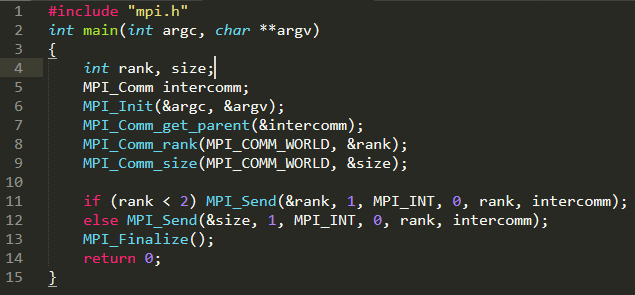
\includegraphics[scale=0.86]{18.slave.code.png}

Assignment 18 - slave code
\end{center}

In this lab there are two programs - master program and slave program. In master program there is a new function: 

\textsc{MPI\_Comm\_spawn}(

\begin{itemize}
	\item IN const char *command - name of program to be spawned (string, significant only at root). In now code our slave program is located in folder \textsc{./cpf/18\_slave.o}.
	\item IN char *argv[] - arguments to command (array of strings, significant only at root)
	\item IN int maxprocs - maximum number of processes to start (integer, significant only at root)
	\item IN MPI\_Info info - a set of key-value pairs telling the runtime system where and how to start the processes (handle, significant only at root)
	\item IN int root - rank of process in which previous arguments are examined (integer)
	\item IN MPI\_Comm comm - intracommunicator containing group of spawning processes (handle)
	\item OUT MPI\_Comm * intercomm - intercommunicator between original group and the newly spawned group (handle)
	\item OUT int array\_of\_errcodes[] - one code per process (array of integer)
\end{itemize}
) which spawn up to \textsc{maxprocs} instances of a single MPI application. In our program the $\operatorname{maxprocs}=3$. After that the slave program starts, in which there are such a simple logic - if rank of processes is lower than $2$ these processes are sending their rank, else process send information about maximum amount of processes in this start. For communication with parent process slaves processes have to user \textsc{MPI\_Comm\_get\_parent} function which returns the parent's process communicator. In master program we expected the results from each processes in variables \textsc{rank1}, \textsc{rank2} and \textsc{total} and after that the results are displayed (as shown on picture higher) - as we expected. Two programs works correctly and understandable.

\newpage

\subsection{Assignment 19. MPI. Dynamic process control. Client-server communication.}

\subsubsection{Formulation of the problem}

To complete the task, you need to create and compile two programs: server and client. In one window of the 
SSH client, a server is launched for one process, which gives out the port name.

An example of a command to start the server: \textsc{mpiexec -n 1 ./serv.o}

Then the client is launched in another window, specifying the port name separated by a space in single quotes 
(example command: \textsc{mpiexec -n 1 ./client.o ‘port name’}).

Understand the new functions in \textsc{Assignment19\_serv.c} and \textsc{Assignment19\_client.c} and explain programs 
execution.

\subsubsection{Example of launch parameters and output. Detailed description of solution}

Code for \textbf{assignment 18} are \href{https:\//github.com/aptmess/parallel_algorithms/blob/master/HT/hw_mpi/Assignment19_serv.c}{here}(server) and \href{https:\//github.com/aptmess/parallel_algorithms/blob/master/HT/hw_mpi/Assignment19_client.c}{here}(client).

Compilation example: 

\begin{enumerate}
	\item \textsc{mpicc.mpich -o ./cpf/19\_serv.o Assignment19\_serv.c}
	\item \textsc{mpicc.mpich -o ./cpf/19\_client.o Assignment19\_client.c}
\end{enumerate}

Firstly we compile two programs with server and client and start a server by command:

\textsc{mpiexec.mpich -np 1 ./cpf/19\_serv.o} - firslt this, then copy the port to client program

\begin{center}
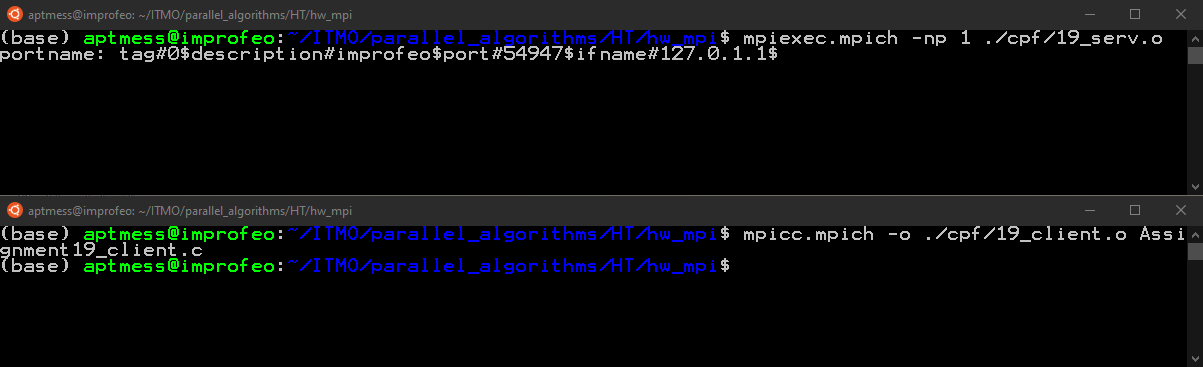
\includegraphics[scale=0.5]{19.before.png}
\end{center}

AFter that we are executing client with port as a parameter: mpiexec.mpich -np 1 ./cpf/19\_client.o 'tag\#0\$description\#improfeo\$port\#50643\$ifname\#127.0.1.1\$' and got results:

\begin{center}
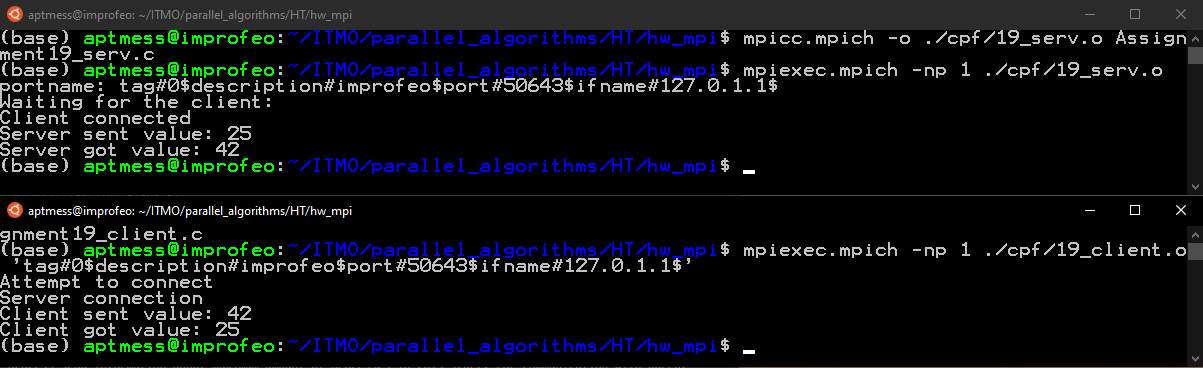
\includegraphics[scale=0.5]{19.after.png}
\end{center}

Let's move to the the code and explain how it works.

\begin{center}
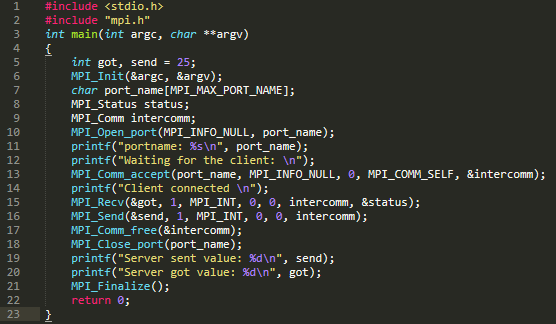
\includegraphics[scale=1.1]{19.serv.code.png}

Assignment 19 - server code
\end{center}

\begin{center}
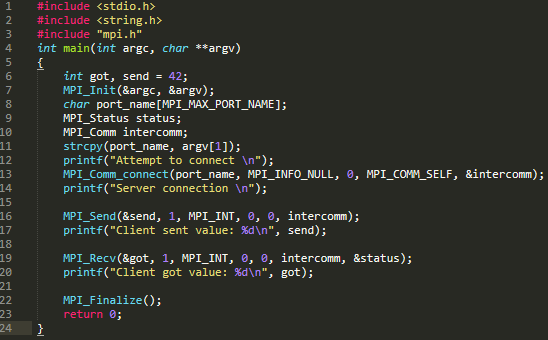
\includegraphics[scale=1.1]{19.client.code.png}

Assignment 19 - client code
\end{center}

In this lab there are a server-client pretty architecture, where firstly in server program with function \textsc{MPI\_Open\_port} establish an address that can be used to establish connections between groups of MPI processes, after that using \textsc{MPI\_Comm\_accept} accept a request to form a communicator and start waiting for the request from client. Then we go to client command and there we establish communication between clien and server using \textsc{MPI\_comm\_connect} by input port and then we send by client a message with value $42$ to server. Server got a request, displayed information about it and send to client server's value - $25$ which is also displayed on client's side. After that the port is closing and the server and client's end's their programs. The results are shown in picture higher and it is expected by us and explained - two programs works correctly.


\subsection{Appendix}
 
The link to the sourse code which is placed on my \href{https://github.com/aptmess/parallel_algorithms}{github}.


\end{document}